\documentclass[10pt,a4paper]{article}

\usepackage{amssymb}
\usepackage[english]{babel}
\usepackage[utf8]{inputenc}
\usepackage{graphicx}
\usepackage{lineno}
\usepackage{cite}
\usepackage{float}
\usepackage{ccaption}
\usepackage{caption}
\usepackage{array}
\usepackage{lscape}
\usepackage[hmargin=2cm,vmargin=2cm]{geometry}
\usepackage{fancyvrb}
\usepackage{hyperref}

\title{{\tt TESS3} reference manual \\
Command-line program and R package
}

\author{
        Kevin Caye (kevin.caye@imag.fr)\\
        Olivier Fran\c cois (olivier.francois@imag.fr)\\
}

\newcommand{\bp}{\mathbf{p}}
\newcommand{\LLL}{\mathcal{L}}

%% BEGIN DOC
\begin{document}


\maketitle
\begin{center}
{\it Please, print this reference manual only if it is necessary.}
\end{center}

\vspace{.5cm}

\begin{center} {\bf Summary}
\end{center}


\vspace{.5cm}

Geography is an important determinant of genetic variation in natural 
populations, and its effects are commonly investigated by analyzing population 
genetic structure using spatial ancestry estimation programs. A common issue is 
that classical spatial ancestry estimation programs do not scale with the 
dimension of the data sets generated from modern sequencing technologies, and 
more efficient algorithms are needed to analyze genome-wide patterns of 
population genetic variation in their geographic context.

The computer program {\tt TESS3} implements admixture models. The program has 
functionalities similar to the previous versions of {\tt 
TESS}~\cite{chen2007bayesian,durand2009spatial}, has run-times several order 
faster than those of common Bayesian clustering programs. In addition, the 
program can be used to perform genome scans for selection based on ancestral 
allele frequency differentiation statistic, and to separate non-adaptive and 
adaptive genetic variation.

This documentation aims to help users to run the {\tt TESS3} command-line engine 
and on Linux, Mac and Windows operating systems. This documentation also presents {\tt tess3r},a R package 
which implements {\tt TESS3} method with some R functions that facilitate the 
post-processing of the program outputs. The main features of {\tt 
TESS3} are illustrated using an example data set, simulated from European lines 
of the plant species {\it Arabidopsis thaliana}.

\vspace{.5cm}


\section{Program installation} 

\subsection{R package}
The installation of {\tt tess3r} R package requires that {\tt R} is install on your computer (\url{ 
https://www.r-project.org/}). You can install the R package directly from the github repository thanks to the package devtools. 
If you don't already have {\tt devtools} R package you can install it from CRAN. In a R session paste this command:

\begin{Verbatim}[frame = single]
install.packages("devtools")
\end{verbatim}


Then, you can install the R package. In a R session paste this command:

\begin{Verbatim}[frame = single]
devtools::install_github("cayek/TESS3/tess3r")
\end{Verbatim}

\subsection{Command-line software} 

The installation of {\tt TESS3} command-line software requires that {\tt CMake}, a the cross-platform 
open-source build system, is installed on the computer OS (\url{ 
http://www.cmake.org/}).  The {\tt TESS3}  program source code can be downloaded 
from the following Github address: \url{https://github.com/cayek/TESS3}. After 
downloading the files as a zipped archive, unzipping the archive will create a 
{\tt TESS3-master} directory on the system. This  directory contains the 
following subdirectories:
\begin{itemize}
\item   {\tt tess3r}: the source code of the program,

\item   {\tt external}: external libraries,

\item     {\tt doc}: the program documentation.

\item     {\tt data}: some simulated data sets for experimenting the program 
use.
\end{itemize}
\noindent The installation of {\tt TESS3} can be performed by typing the 
following instructions in a terminal session from the {\tt TESS3-master} 
directory.

\begin{Verbatim}[frame = single]
 mkdir build/
 cd build/
 cmake -DCMAKE_BUILD_TYPE=release ../
 make TESS3
\end{Verbatim}

 \noindent The executable program file {\tt TESS3} will be found in the {\tt 
build} directory. Copy this file to the \verb|TESS3-master| directory, and 
change directory to the main directory.
 
\section{Data format}

\subsection{Input files}

{\tt TESS3} requires two input files, the first one recording individual 
genotype data and the second one containing the geographic coordinates of  each 
sampled individual. For organism genomes of arbitrary ploidy, the standard data 
type for {\tt TESS3} is the {\bf single nucleotide polymorphism} (SNP) type.  
The genotype matrix must be formatted in the {\bf geno} format and the 
coordinate file must be formatted in the {\bf coord} format.

Users who want to process allelic data, such as microsatellite markers or AFLPs, 
and have their data in the {\tt TESS} 2.3 format can also use {\tt TESS3}. They 
need to convert their data in the geno+coord data format, and can do this using 
the {\tt tess2tess3} function implemented in the {\tt R} script {\tt 
src/Rwrapper/TESS3.R}.




\begin{itemize}
\item {\bf geno} (example.geno)

The {\bf geno} format has one row for each SNP. Each row contains 1 character 
per individual. For diploid genomes,  0 means zero copies of the reference 
allele, 1 means one copy of the reference allele, 2 means two copies of the 
reference allele, and 9 codes for some missing data. Here is an example of a 
geno file for $n=3$ individuals and $L=4$ loci.
\\
\begin{center}
\footnotesize
\begin{Verbatim}[frame=single]
112
010
091
121
\end{Verbatim}
\end{center}


\item {\bf coord} (example.coord)

The {\bf coord} format has one row for each individual. Each row contains the 
\verb|longitude| and \verb|latitude| coordinates of each individual.
\\
\begin{center}
\footnotesize
\begin{Verbatim}[frame=single]
2.5154 5.4390
-8.4293 4.0197
1.3536 5.5852
\end{Verbatim}
\end{center}

\end{itemize}

\noindent Users having their genotype data in the {\bf ped}, {\bf ancestrymap}, 
{\bf vcf} or {\bf lfmm} format  can use the {\tt R} package {\tt LEA} to convert 
them in the {\bf geno} format~\cite{frichot2015lea}. 

\subsection{Output files}

{\tt TESS3} produces three main {\bf output files}:

\begin{itemize}
\item The file with the extension the {\bf .K.Q} contains the $Q$-matrix of 
individual ancestry coefficients.
The $Q$-matrix has $n$ rows (the number of individuals) and $K$ columns (the 
number of ancestral populations).
\item The file with the extension {\bf K.G} contains the $G$-matrix of ancestral 
genotype frequencies.
The $G$-matrix has $N_g\times L$ lines (the number of genotypes times the number 
of SNPs) and $K$ columns (the number of ancestral populations). For diploid 
organisms, the first row represents the frequencies of genotype 0 in each 
ancestral population, the second row represents the frequencies of genotype 1, 
and the third line the ancestral frequencies of 2.
\item The file with the extension {\bf .Fst} contains the values of the 
ancestral allele frequency differentiation statistic $F_{\rm ST}$ computed at 
each locus.  
\end{itemize}

There are additional {\bf output files} that are useful to get information about 
the nearest-neighbor graph, the least-squares error and the cross-entropy 
criterion computed by the program.

\begin{itemize}
\item The file with the extension {\bf .W} contains weight matrix for the 
nearest-neighbor graph.
\item The file with the extension the {\bf .sum} contains the values of the 
least-squares error, the cross-entropy criterion computed with all the data and 
with a percentage of masked data when the user asks the program to compute it.
\end{itemize}

\section{R package}

\subsection{Tutorial}
We advice to start with the R package tutorials which can be found here: \url{https://
github.com/cayek/TESS3/blob/master/doc/tess3r_tutorial.html}.

\subsection{Documentation}
The complete documentation of the package is available following this link: \url{https://
github.com/cayek/TESS3/blob/master/doc/tess3r.pdf}.


\section{Run the command-line program}
\subsection{Command-line}
The {\tt TESS3} program can be executed from a command line. The basic format is 
as follows
\begin{Verbatim}[frame=single]
./TESS3 -x genotype_file.geno  -r coordinates_file.coord -K 
number_of_ancestral_populations
\end{Verbatim}

\noindent
Only the three options {\tt -x -r -K}  are mandatory. The ordering of the 
options in the command line is unimportant. Here is a description of these 
options:
\begin{itemize}
\item \verb|-x genotype_file.geno| is the path to the genotype file (in the 
.geno format),
\item \verb|-r coordinates_file.coord| is the path to the coordinate file (in 
the .coord format),
\item \verb|-K number_of_ancestral_populations| is the number of ancestral 
populations.
\end{itemize}

\noindent
Some additional options are available:
\begin{itemize}
\item \verb|-m ploidy|  1 if haploid, 2 if diploid (default: 2). 
\item \verb|-a alpha| is the value of the normalized regularization parameter 
(default: 0.001). This parameter controls the geographic regularity of ancestry 
estimates.
\item \verb|-W edge_weight_input| is the path to a file that contains a 
pre-specified edge weight matrix for the nearest-neighbor graph (separator = 
space character). The program uses this matrix when the option is set, otherwise 
it uses the default values.
\item \verb|-q output_Q| is a path for the output file containing the $Q$-matrix 
of ancestry coefficients. The default name of the output file is the same name 
as the input file with the extension {\tt .K.Q}.
\item \verb|-g output_G| is a path to the output file containing the ancestral 
genotype frequencies. The default name of the output file is the same name as 
the input genotype file with the extension {\tt .K.G}.
\item \verb|-f output_FST| is a path to the output file containing the values of 
the ancestral allele frequency differentiation statistic for each loci. The 
default name of the output file is the same name as the input genotype file with 
the extension {\tt .K.Fst}.
\item \verb|-y output_sum| is a path to the output file containing the value of 
the least-squares criterion, the cross-entropy criteria on all data and on 
masked data only. By default, the name of the output file is the same name as 
the input genotype file with the extension {\tt .K.sum}.
\item \verb|-c perc| is the percentage of masked genotypes. If this option is 
set, the cross-entropy criterion is computed (see\cite{frichot2014fast} for more 
details on the cross-entropy criterion). The default percentage is $0.05$.
\item \verb|-e tolerance| is the tolerance error in the optimization algorithm 
(by default: 0.0000001). 
\item \verb|-i iteration_number| is the maximum number of iterations of the 
algorithm (default: 200). 
\item \verb|-I nb_SNPs| starts the algorithm with a run using a subset of 
nb\_SNPs random SNPs. This option speeds up the estimation algorithm for very 
large data sets.
\item \verb|-Q input_Q| is the path to an initial file for the $Q$ matrix 
containing individual ancestry coefficients. If both \verb|-I| and \verb|-Q| are 
set, \verb|-Q| is chosen.
\item \verb|-s seed| is a seed to initialize the random number generator. 
\item \verb|-p p| is the number of CPUs to use when the algorithm is run on a 
multiprocessor system.
Be aware that the number of processes has to be lower or equal to the number of 
CPU units available on your computer (default: 1).

\end{itemize}


\noindent A summary of options can be obtained  by typing the following command
\footnotesize
\begin{Verbatim}[frame=single]
./TESS3 -h
\end{Verbatim}
\noindent
\normalsize


\subsection{Example}\label{sec:ex}

To run a very simple example of the use of {\tt TESS3}, consider data simulated 
from the chromosome 5 of the model plant species {\it A. thaliana}. The genotype 
matrix contains 170 genotypes from European lines of the plant (26943 SNPs). 
Since {\it A. thaliana} is a selfing species, the heterozygote frequency was 
equal to zero, and the diploid genotypes were recoded as haploid. Copy the 
program executable file in the {\tt ./data/simulated/Athaliana} directory and 
type

\begin{Verbatim}[frame=single]
./TESS3 -x Athaliana.geno  -r Athaliana.coord -K 3 -m 1
\end{Verbatim}

\noindent Then, open a {\tt R} session and type


\begin{Verbatim}[frame=single]
> par( mfrow = c(2,1) )
> Qmatrix = t( read.table("Athaliana.3.Q") )
> barplot(Qmatrix, col = 2:4)
> Fst = read.table("Athaliana.3.Fst")[,1]
> plot(Fst, main = "Manhattan Plot", cex = .4, pch = 19, col = "blue")
\end{Verbatim}

Those commands visualize the ancestry coefficient matrix computed by {\tt TESS3} 
and display a Manhattan plot of $F_{\rm ST}$ values along the fifth chromosome 
of the plant species (figure~\ref{fig:bar}).


\begin{figure}[h!]\centering
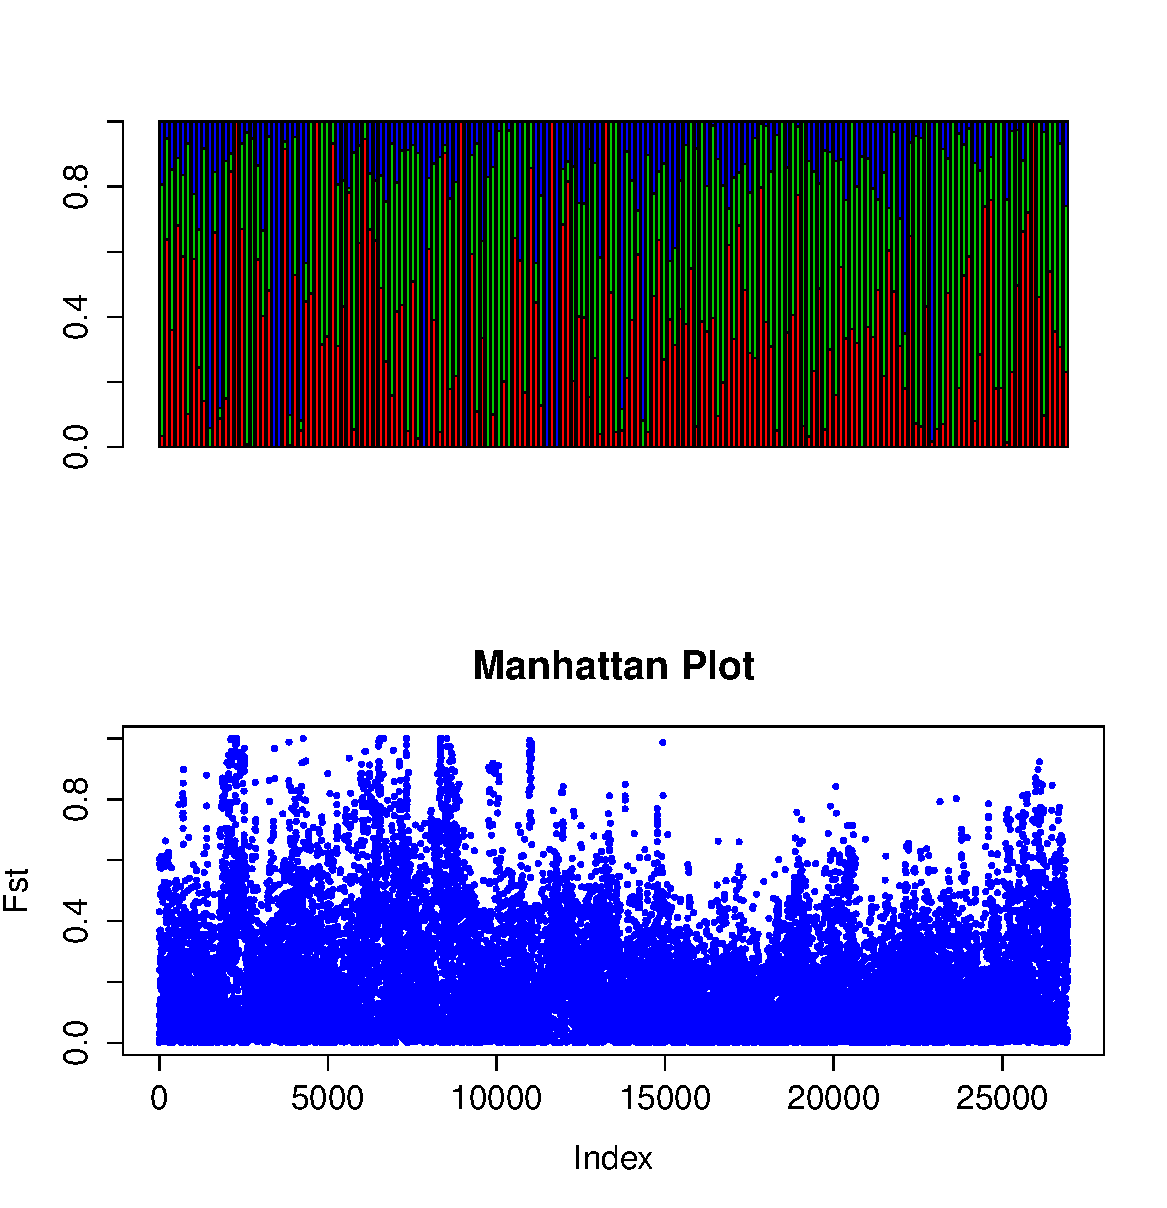
\includegraphics[width=\linewidth]{barplot.pdf}
\caption{Results of the {\tt R} commands of section 3.2.}\label{fig:bar}
\end{figure} 

\section{Contact}
If you need assistance, do not hesitate to send us an email (kevin.caye@imag.fr 
or olivier.francois@imag.fr). 

\bibliographystyle{plain}
\bibliography{note}

\end{document}
